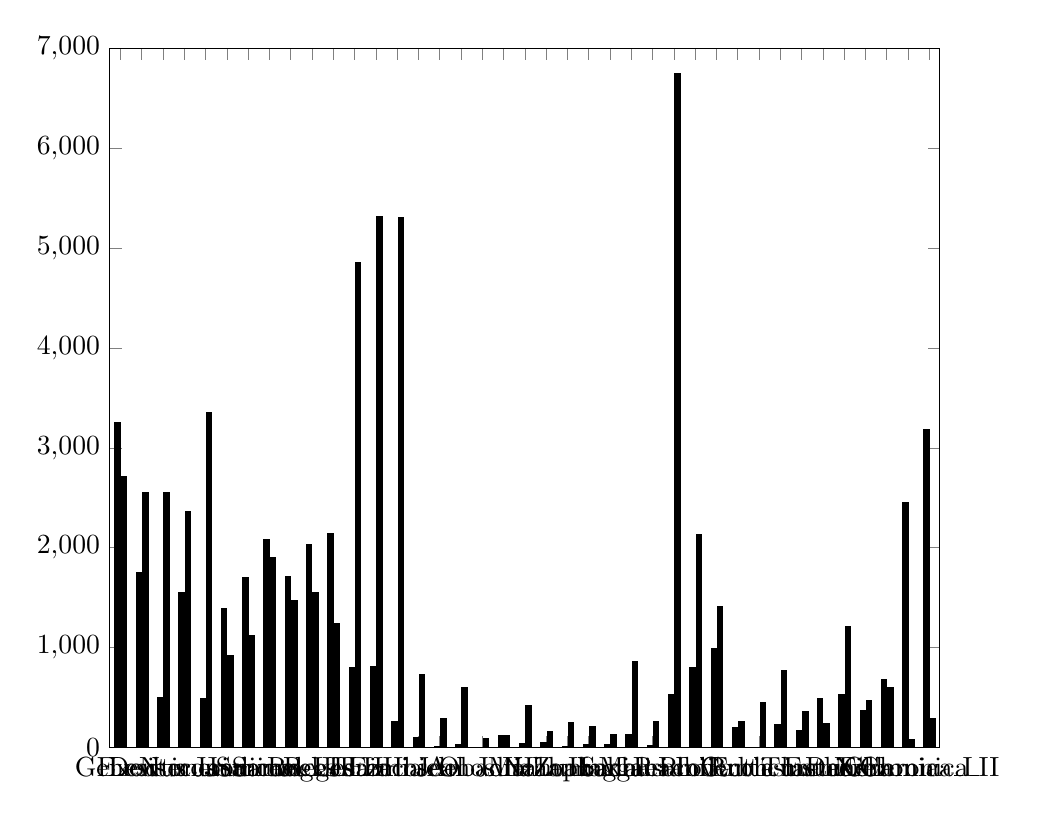
\begin{tikzpicture}[baseline]
\begin{axis}[
width=\textwidth,
xmin=-0.5, xmax=38.5,
ymin=0, ymax=7000,
xtick={0,1,2,3,4,5,6,7,8,9,10,11,12,13,14,15,16,17,18,19,20,21,22,23,24,25,26,27,28,29,30,31,32,33,34,35,36,37,38},
xticklabels={Genesis,Exodus,Leviticus,Numeri,Deuteronomium,Josua,Judices,Samuel\_I,Samuel\_II,Reges\_I,Reges\_II,Jesaia,Jeremia,Ezechiel,Hosea,Joel,Amos,Obadia,Jona,Micha,Nahum,Habakuk,Zephania,Haggai,Sacharia,Maleachi,Psalmi,Iob,Proverbia,Ruth,Canticum,Ecclesiastes,Threni,Esther,Daniel,Esra,Nehemia,Chronica\_I,Chronica\_II},
xticklabel style = {\xticklabel},
]
\draw[draw=\bardrawcolor,fill=\barcolor] (axis cs:-0.25,0) rectangle (axis cs:0,3249);
\draw[draw=\bardrawcolor,fill=\barcolorr] (axis cs:0.05,0) rectangle (axis cs:0.3,2711);
\draw[draw=\bardrawcolor,fill=\barcolor] (axis cs:0.75,0) rectangle (axis cs:1,1750);
\draw[draw=\bardrawcolor,fill=\barcolorr] (axis cs:1.05,0) rectangle (axis cs:1.3,2557);
\draw[draw=\bardrawcolor,fill=\barcolor] (axis cs:1.75,0) rectangle (axis cs:2,501);
\draw[draw=\bardrawcolor,fill=\barcolorr] (axis cs:2.05,0) rectangle (axis cs:2.3,2554);
\draw[draw=\bardrawcolor,fill=\barcolor] (axis cs:2.75,0) rectangle (axis cs:3,1551);
\draw[draw=\bardrawcolor,fill=\barcolorr] (axis cs:3.05,0) rectangle (axis cs:3.3,2359);
\draw[draw=\bardrawcolor,fill=\barcolor] (axis cs:3.75,0) rectangle (axis cs:4,494);
\draw[draw=\bardrawcolor,fill=\barcolorr] (axis cs:4.05,0) rectangle (axis cs:4.3,3351);
\draw[draw=\bardrawcolor,fill=\barcolor] (axis cs:4.75,0) rectangle (axis cs:5,1391);
\draw[draw=\bardrawcolor,fill=\barcolorr] (axis cs:5.05,0) rectangle (axis cs:5.3,925);
\draw[draw=\bardrawcolor,fill=\barcolor] (axis cs:5.75,0) rectangle (axis cs:6,1706);
\draw[draw=\bardrawcolor,fill=\barcolorr] (axis cs:6.05,0) rectangle (axis cs:6.3,1119);
\draw[draw=\bardrawcolor,fill=\barcolor] (axis cs:6.75,0) rectangle (axis cs:7,2086);
\draw[draw=\bardrawcolor,fill=\barcolorr] (axis cs:7.05,0) rectangle (axis cs:7.3,1904);
\draw[draw=\bardrawcolor,fill=\barcolor] (axis cs:7.75,0) rectangle (axis cs:8,1711);
\draw[draw=\bardrawcolor,fill=\barcolorr] (axis cs:8.05,0) rectangle (axis cs:8.3,1469);
\draw[draw=\bardrawcolor,fill=\barcolor] (axis cs:8.75,0) rectangle (axis cs:9,2033);
\draw[draw=\bardrawcolor,fill=\barcolorr] (axis cs:9.05,0) rectangle (axis cs:9.3,1551);
\draw[draw=\bardrawcolor,fill=\barcolor] (axis cs:9.75,0) rectangle (axis cs:10,2144);
\draw[draw=\bardrawcolor,fill=\barcolorr] (axis cs:10.05,0) rectangle (axis cs:10.3,1236);
\draw[draw=\bardrawcolor,fill=\barcolor] (axis cs:10.75,0) rectangle (axis cs:11,801);
\draw[draw=\bardrawcolor,fill=\barcolorr] (axis cs:11.05,0) rectangle (axis cs:11.3,4854);
\draw[draw=\bardrawcolor,fill=\barcolor] (axis cs:11.75,0) rectangle (axis cs:12,805);
\draw[draw=\bardrawcolor,fill=\barcolorr] (axis cs:12.05,0) rectangle (axis cs:12.3,5319);
\draw[draw=\bardrawcolor,fill=\barcolor] (axis cs:12.75,0) rectangle (axis cs:13,257);
\draw[draw=\bardrawcolor,fill=\barcolorr] (axis cs:13.05,0) rectangle (axis cs:13.3,5303);
\draw[draw=\bardrawcolor,fill=\barcolor] (axis cs:13.75,0) rectangle (axis cs:14,96);
\draw[draw=\bardrawcolor,fill=\barcolorr] (axis cs:14.05,0) rectangle (axis cs:14.3,732);
\draw[draw=\bardrawcolor,fill=\barcolor] (axis cs:14.75,0) rectangle (axis cs:15,11);
\draw[draw=\bardrawcolor,fill=\barcolorr] (axis cs:15.05,0) rectangle (axis cs:15.3,292);
\draw[draw=\bardrawcolor,fill=\barcolor] (axis cs:15.75,0) rectangle (axis cs:16,33);
\draw[draw=\bardrawcolor,fill=\barcolorr] (axis cs:16.05,0) rectangle (axis cs:16.3,603);
\draw[draw=\bardrawcolor,fill=\barcolor] (axis cs:16.75,0) rectangle (axis cs:17,1);
\draw[draw=\bardrawcolor,fill=\barcolorr] (axis cs:17.05,0) rectangle (axis cs:17.3,84);
\draw[draw=\bardrawcolor,fill=\barcolor] (axis cs:17.75,0) rectangle (axis cs:18,115);
\draw[draw=\bardrawcolor,fill=\barcolorr] (axis cs:18.05,0) rectangle (axis cs:18.3,116);
\draw[draw=\bardrawcolor,fill=\barcolor] (axis cs:18.75,0) rectangle (axis cs:19,35);
\draw[draw=\bardrawcolor,fill=\barcolorr] (axis cs:19.05,0) rectangle (axis cs:19.3,421);
\draw[draw=\bardrawcolor,fill=\barcolor] (axis cs:19.75,0) rectangle (axis cs:20,47);
\draw[draw=\bardrawcolor,fill=\barcolorr] (axis cs:20.05,0) rectangle (axis cs:20.3,159);
\draw[draw=\bardrawcolor,fill=\barcolor] (axis cs:20.75,0) rectangle (axis cs:21,4);
\draw[draw=\bardrawcolor,fill=\barcolorr] (axis cs:21.05,0) rectangle (axis cs:21.3,250);
\draw[draw=\bardrawcolor,fill=\barcolor] (axis cs:21.75,0) rectangle (axis cs:22,27);
\draw[draw=\bardrawcolor,fill=\barcolorr] (axis cs:22.05,0) rectangle (axis cs:22.3,206);
\draw[draw=\bardrawcolor,fill=\barcolor] (axis cs:22.75,0) rectangle (axis cs:23,25);
\draw[draw=\bardrawcolor,fill=\barcolorr] (axis cs:23.05,0) rectangle (axis cs:23.3,133);
\draw[draw=\bardrawcolor,fill=\barcolor] (axis cs:23.75,0) rectangle (axis cs:24,124);
\draw[draw=\bardrawcolor,fill=\barcolorr] (axis cs:24.05,0) rectangle (axis cs:24.3,861);
\draw[draw=\bardrawcolor,fill=\barcolor] (axis cs:24.75,0) rectangle (axis cs:25,14);
\draw[draw=\bardrawcolor,fill=\barcolorr] (axis cs:25.05,0) rectangle (axis cs:25.3,260);
\draw[draw=\bardrawcolor,fill=\barcolor] (axis cs:25.75,0) rectangle (axis cs:26,529);
\draw[draw=\bardrawcolor,fill=\barcolorr] (axis cs:26.05,0) rectangle (axis cs:26.3,6747);
\draw[draw=\bardrawcolor,fill=\barcolor] (axis cs:26.75,0) rectangle (axis cs:27,800);
\draw[draw=\bardrawcolor,fill=\barcolorr] (axis cs:27.05,0) rectangle (axis cs:27.3,2132);
\draw[draw=\bardrawcolor,fill=\barcolor] (axis cs:27.75,0) rectangle (axis cs:28,991);
\draw[draw=\bardrawcolor,fill=\barcolorr] (axis cs:28.05,0) rectangle (axis cs:28.3,1409);
\draw[draw=\bardrawcolor,fill=\barcolor] (axis cs:28.75,0) rectangle (axis cs:29,199);
\draw[draw=\bardrawcolor,fill=\barcolorr] (axis cs:29.05,0) rectangle (axis cs:29.3,257);
\draw[draw=\bardrawcolor,fill=\barcolor] (axis cs:29.75,0) rectangle (axis cs:30,2);
\draw[draw=\bardrawcolor,fill=\barcolorr] (axis cs:30.05,0) rectangle (axis cs:30.3,454);
\draw[draw=\bardrawcolor,fill=\barcolor] (axis cs:30.75,0) rectangle (axis cs:31,233);
\draw[draw=\bardrawcolor,fill=\barcolorr] (axis cs:31.05,0) rectangle (axis cs:31.3,767);
\draw[draw=\bardrawcolor,fill=\barcolor] (axis cs:31.75,0) rectangle (axis cs:32,164);
\draw[draw=\bardrawcolor,fill=\barcolorr] (axis cs:32.05,0) rectangle (axis cs:32.3,360);
\draw[draw=\bardrawcolor,fill=\barcolor] (axis cs:32.75,0) rectangle (axis cs:33,486);
\draw[draw=\bardrawcolor,fill=\barcolorr] (axis cs:33.05,0) rectangle (axis cs:33.3,241);
\draw[draw=\bardrawcolor,fill=\barcolor] (axis cs:33.75,0) rectangle (axis cs:34,534);
\draw[draw=\bardrawcolor,fill=\barcolorr] (axis cs:34.05,0) rectangle (axis cs:34.3,1212);
\draw[draw=\bardrawcolor,fill=\barcolor] (axis cs:34.75,0) rectangle (axis cs:35,373);
\draw[draw=\bardrawcolor,fill=\barcolorr] (axis cs:35.05,0) rectangle (axis cs:35.3,469);
\draw[draw=\bardrawcolor,fill=\barcolor] (axis cs:35.75,0) rectangle (axis cs:36,683);
\draw[draw=\bardrawcolor,fill=\barcolorr] (axis cs:36.05,0) rectangle (axis cs:36.3,598);
\draw[draw=\bardrawcolor,fill=\barcolor] (axis cs:36.75,0) rectangle (axis cs:37,2448);
\draw[draw=\bardrawcolor,fill=\barcolorr] (axis cs:37.05,0) rectangle (axis cs:37.3,74);
\draw[draw=\bardrawcolor,fill=\barcolor] (axis cs:37.75,0) rectangle (axis cs:38,3184);
\draw[draw=\bardrawcolor,fill=\barcolorr] (axis cs:38.05,0) rectangle (axis cs:38.3,292);
\end{axis}
\end{tikzpicture}

